%    This program is free software: you can redistribute it and/or modify
%    it under the terms of the GNU General Public License as published by
%    the Free Software Foundation, either version 3 of the License, or
%    (at your option) any later version.
%
%    This program is distributed in the hope that it will be useful,
%    but WITHOUT ANY WARRANTY; without even the implied warranty of
%    MERCHANTABILITY or FITNESS FOR A PARTICULAR PURPOSE.  See the
%    GNU General Public License for more details.
%
%    You should have received a copy of the GNU General Public License
%    along with this program.  If not, see <http://www.gnu.org/licenses/>.\documentclass[a4paper,11pt]{article}
%
%    Copyright: John A Stevenson, University of Edinburgh, Twitter: @volcan01010

\documentclass[a4paper,11pt]{article}

%%%%%%%%%%% PAGE SIZE: Set up page with 2 cm margins
\usepackage{anysize}
\marginsize{2cm}{2cm}{2cm}{0cm}

%%%%%%%%%%% FONTS:
\usepackage[icelandic,english]{babel} % Font encoding for Icelandic characters
\usepackage[T1]{fontenc} % Font encoding for Icelandic characters
\usepackage{textgreek} % Greek letters without going into Math mode
\usepackage{eulervm} % This makes mathtext upright, not italic

\usepackage[scaled]{helvet} % Helvetica.  Similar to Arial as specified by NERC
\renewcommand*{\familydefault}{\sfdefault} % Helvetica needs default font to be SansSerif
%\usepackage{libertine} % Linux Libertine font is a nice serif font
%\usepackage{lmodern} % use Latin Modern for that LaTeX look

%%%%%%%%%%% REFERENCES: 
\usepackage[round]{natbib} % Bibliography / reference package
\usepackage{multicol} % Make reference list multicolumn

%%%%%%%%%%% FIGURES:
\usepackage{graphicx} % Includes graphics
\usepackage{float} % Allows forcing of figure locations
\usepackage{wrapfig} % Wraps text round images
% Change figure caption font
\usepackage[font=small,format=plain,labelfont=bf,up,textfont=it,up]{caption}

%%%%%%%%%%% SPACE SAVERS:
\usepackage{mdwlist} % less gaps in itemize sections
\usepackage{titlesec} % format of section titles
\titlespacing{\section}{0pt}{8pt}{4pt}
\titlespacing{\subsection}{0pt}{6pt}{2pt}
%\usepackage{setspace}
%\onehalfspacing
\linespread{0.96}

\setlength{\headheight}{0cm}
\setlength{\headsep}{0cm}
\setlength{\footskip}{0.6cm}
\setlength{\bibsep}{0pt}
\setlength{\parskip}{0.5\parskip}
\setlength{\textfloatsep}{0.5\textfloatsep}

%%%%%%%%%%% OTHER:
\usepackage[hidelinks]{hyperref} % Hyperlinks in pdf (remove 'hidelinks' to display)
\usepackage[dvipscolors]{xcolor}

% Gantt chart package
\usepackage{pgfgantt}

%% The lineno packages adds line numbers. Start line numbering with
%% \begin{linenumbers}, end it with \end{linenumbers}. Or switch it on
%% for the whole article with \linenumbers.
\usepackage[modulo]{lineno}

\title{Gas, not ice, makes subglacial rhyolite explode}
\author{Dr John A Stevenson}
\date{\today}

\begin{document}
%%%%%%%%%%%%%%%%%%%%%%%%%%%%%%%%%%%%%%%%%%%%%%%%%%%%%%%%%%%%%%%%%
\begin{center}
	{\LARGE Gas, not ice, makes subglacial rhyolite explode}
\end{center}
\smallskip
\hrule height 1pt 

%%%%%%%%%%%%%%%%%%%%%%%%%%%%%%%%%%%%%%%%%%%%%%%%%%%%%%%%%%%%%%%%%
\section*{Outline}
\begin{quote}
\textit{A recent study by Jacqui Owen (Lancaster University), Hugh Tuffen and Dave McGarvie shows that the explosivity of a subglacial rhyolite eruption is determined while the magma is still deep beneath the ground. Rhyolite is a particularly thick and gloopy (viscous) type of magma that is especially prone to explosive eruptions.  I'm really pleased to see this study published because I worked on subglacial rhyolite eruptions for my PhD. Where I mapped and measured pumice deposits to show that whether an eruption is explosive or not is not controlled by the ice, Jacqui has used geochemical methods to show what does control it: dissolved volcanic gases.  Explaining how she found out is also a good excuse to discuss a key question in volcanology: Why do volcanoes explode?} 
\end{quote}
\rule{\textwidth}{1pt}

%%%%%%%%%%%%%%%%%%%%%%%%%%%%%%%%%%%%%%%%%%%%%%%%%%%%%%%%%%%%%%%%%
\section{Volcanoes, explosions and ice}
%-----------------------------------------
\subsection{Why do volcanoes explode?}

% Wrapfigures work best if you force their position at the start of the paragraph that you want them beside.
%\begin{figure}[!h]
\begin{wrapfigure}{r}{0.5\textwidth}
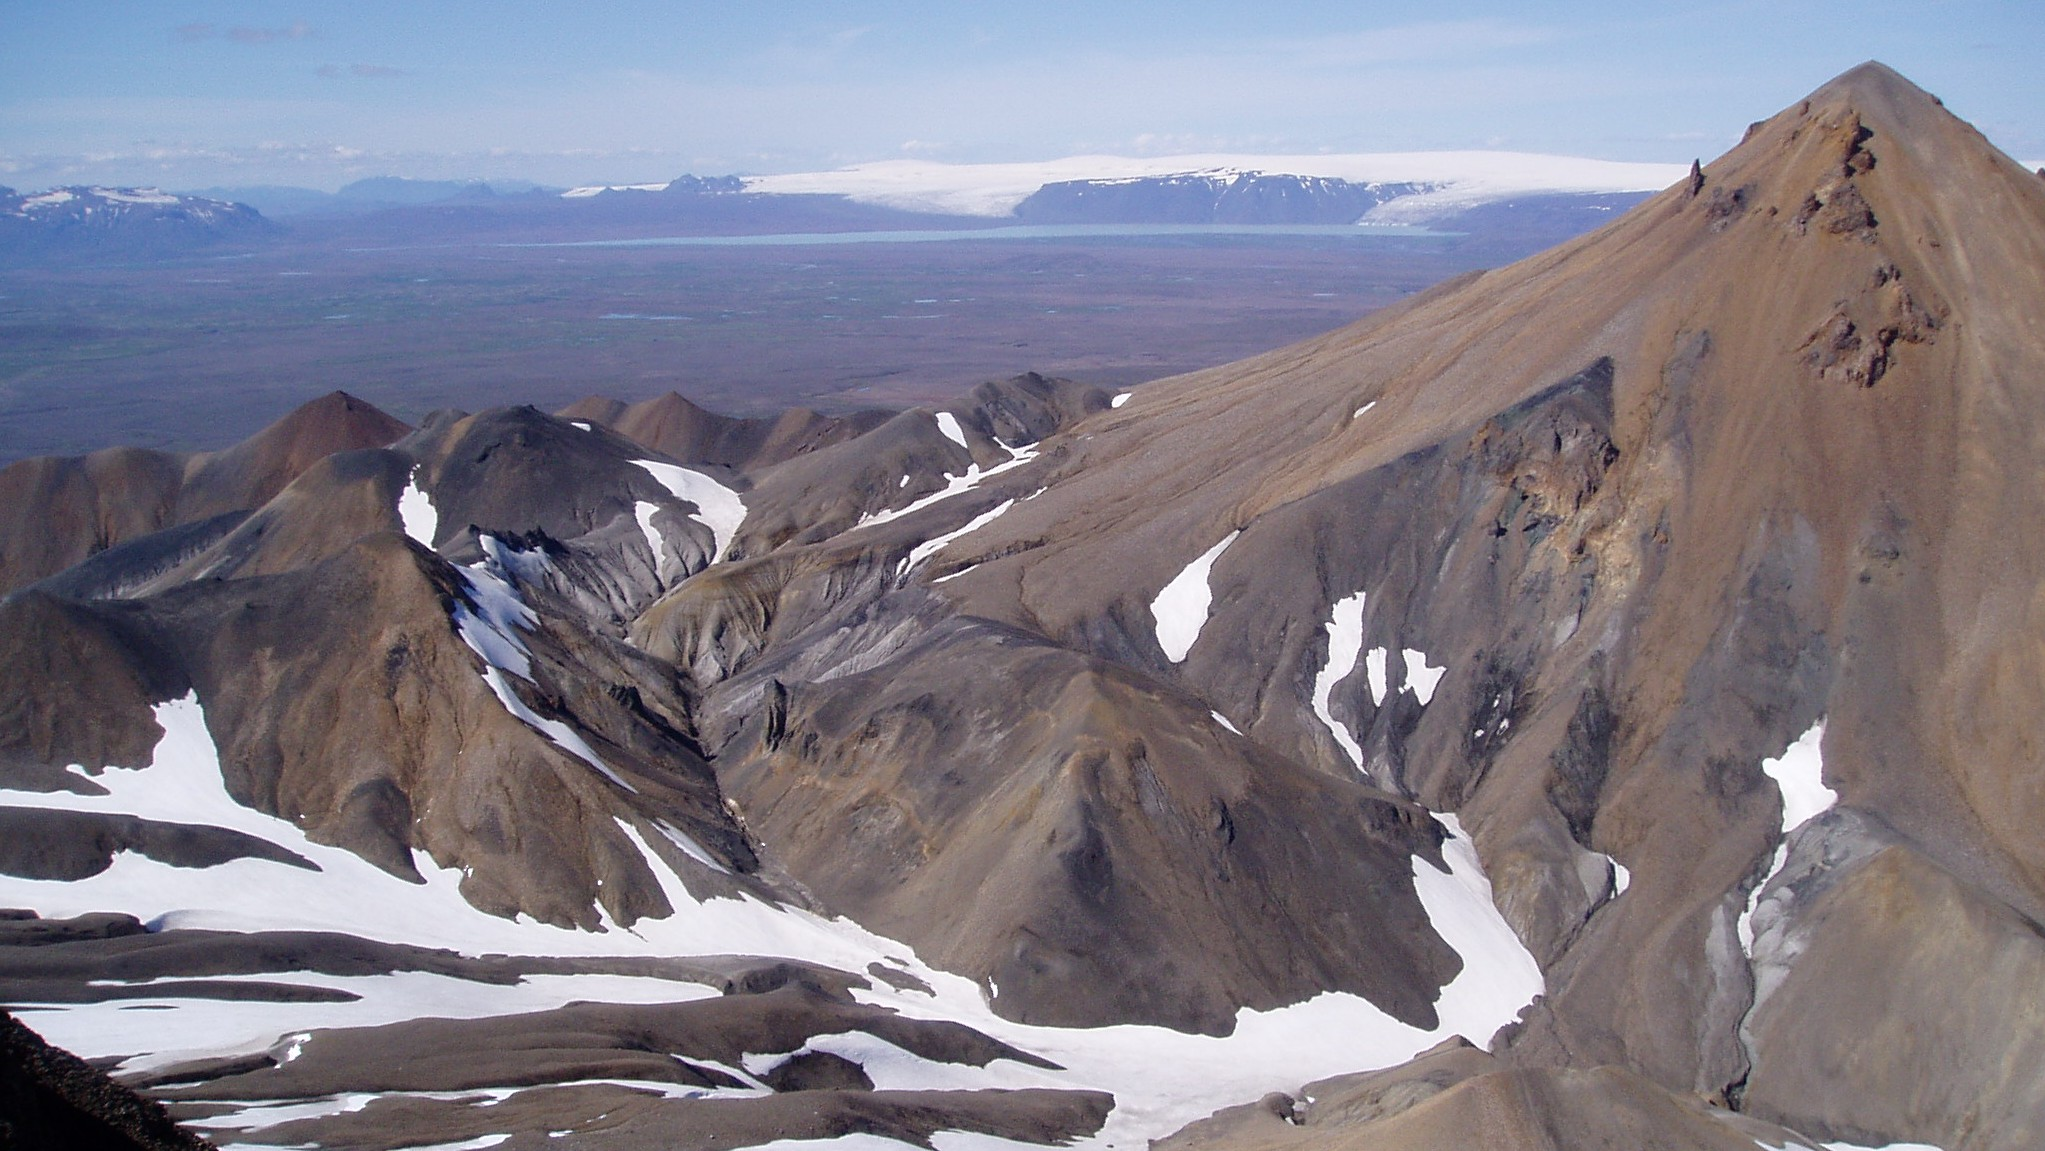
\includegraphics[width=0.49\textwidth]{figures/kerlingarfjoll.jpg}
	\caption{Part of the subglacial rhyolite volcano of Kerlingarfj\"oll, Iceland. Steep mountains like this, dominated by scree, pumice and ash were formed by explosive volcanic eruptions at times when all of Iceland was buried by ice up to 1000 m thick. Water from melting ice is known to make volcanic eruptions more explosive, but recent findings show that the effect is minor in subglacial rhyolite eruptions.}	
	\label{fig:kerlingarfjoll}
\end{wrapfigure}
%\end{figure}

During an explosive eruption, pumice, ash and rock fragments (collectively known as tephra) are blasted from the volcano at high speed, driven by hot, expanding gases. The gases, mainly steam (i.e. water; H$_2$O), have come from within the magma itself. Down in the magma chamber, deep beneath the volcano, the pressure of the weight of the rocks above keeps the gases dissolved, but when the liquid magma rises to the surface, the pressure that it feels decreases. The gases come out of the liquid and form bubbles, just as bubbles appear when you open a bottle of Irn Bru (other, less region-specific, fizzy soft drinks are available). The closer to the surface the magma gets, the more gas comes out, changing the magma from a thick, gloopy liquid, to a thick, gloopy, bubbly liquid, then to a thick, gloopy foam.

Imagine that the conduit (or pathway) through the rocks from the magma chamber to the surface is a rigid pipe, where the same mass of material that enters that bottom (as magma with gas dissolved inside) has to come out at the top (as magma + gas bubbles). This is a closed system. If the volume of a parcel of magma is doubled by forming bubbles, then the speed that it comes out the top must also double. Thus the magma accelerates. Triple the volume, triple the speed.  Quadruple the volume, quadruple the speed. The formation and expansion of gas bubbles drives the magma faster and faster to the surface.

This type of acceleration by expansion is perfectly illustrated by Diet Coke and Mentos eruptions, but volcanoes take things a step further. Once the magma reaches about 70\% bubbles, the forces due to acceleration within the conduit become too much for the foam, which rips or shatters into fragments of pumice and ash. The full power of the gas expansion is now unleashed, no-longer limited by the flow rate of the thick, gloopy magma; the mixture accelerates ferociously. When it comes thundering out at the surface, it is travelling at speeds of over 300 metres per second (1000 km/h, 670 mph).

Explosive eruptions are most common where the magma is so thick and gloopy (viscous) that gas bubbles cannot escape. This is most common with andesite, dacite and rhyolite magma types. The duration of these explosive eruptions depends on the availability of gas-rich magma in the magma chamber.

%-----------------------------------------
\subsection{How does ice affect eruptions?}
\label{sec:surtsey}

It is possible to make an eruption become explosive by adding water. The boiling point of water is well below that of magma (800-1000$^{\circ}$C) and turning water into steam at atmospheric pressure involves a 1000$\times$ increase in volume. This can drive an explosive expansion that fragments magma into pumice and ash. The formation of the island of Surtsey, which grew out of the North Atlantic in 1963-1967, is a good example of an eruption of runny basalt magma that has explosive phases only when water mixed with magma at the vent.

%\begin{figure}[!h]
\begin{wrapfigure}[31]{l}{0.4\textwidth}
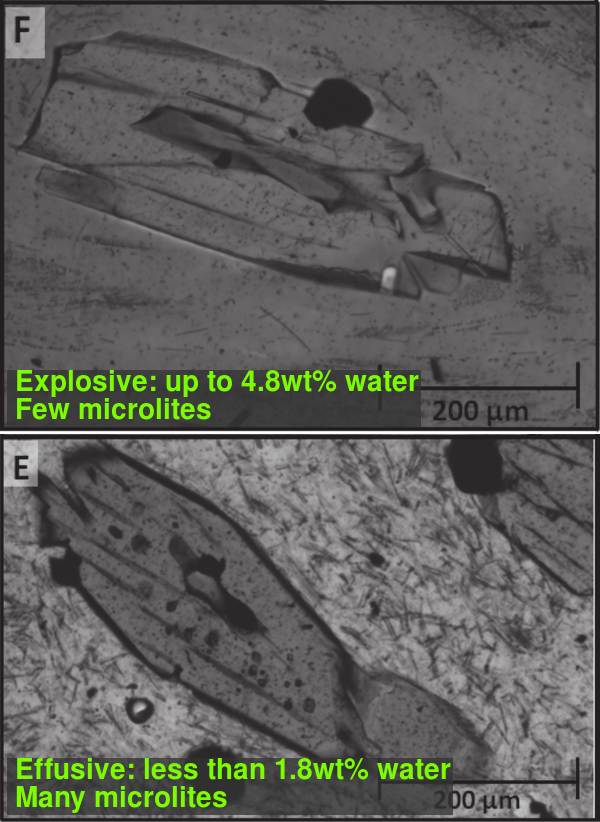
\includegraphics[width=0.39\textwidth]{figures/m_both.png}
	\caption{Microscope images of subglacial rhyolite ash from explosive and effusive eruptions. Owen and coworkers found pockets of frozen melt trapped within the big crystals. These could be analysed to see how much magmatic water was in the magma chamber. Tiny crystals, called microlites, are found in samples from effusive eruptions. They formed as magma moved slowly to the surface, losing gas on the way. Image modified from article in Geology.}	
	\label{fig:inclusions}
\end{wrapfigure}
%\end{figure}

In Iceland, most subglacial eruptions are basaltic. Melting ice adds water to the magma, turning the eruptions explosive.  The eruptions often take place within ice-dammed meltwater lakes.  If the volcano builds above the water surface, Surtsey-like, or if the lake level drops below the vent, then the eruption switches from explosive to effusive (lava-producing). Ice and meltwater therefore control the explosivity of subglacial basalt eruptions and the duration of the explosive phase of an eruption depends on the access of water to the vent.

More recently, researchers have investigated whether the same is true for rhyolite.


%%%%%%%%%%%%%%%%%%%%%%%%%%%%%%%%%%%%%%%%%%%%%%%%%%%%%%%%%%%%%%%%%
\section{Subglacial rhyolite and volcanic gas}
%-----------------------------------------
\subsection{Magma chamber water content}
\label{sec:chamber}

Owen and coworkers sampled 5 different subglacial rhyolite mountains in Torfaj\"okull, Iceland \citet{owen_explosive_2012}.  The first two were piles of pumice, ash and scree up to 1 cubic kilometre in volume, so we know that they formed in large, explosive eruptions. Two were made of lava and were formed in effusive eruptions, and the fifth one was produced by an eruption with both explosive and effusive parts.  The samples contained big crystals (called phenocrysts) that formed in the magma chamber. Some of these had grown in a way that trapped little blobs of melt inside them. These are called melt inclusions and they act as a record of the magma composition before the eruption.

Owen analysed how much water was dissolved in the magma within the melt inclusions.  She found that the samples from the explosive eruptions contained the most (up to 3.9 wt\%; Figure \ref{fig:inclusions}).  A sample from the explosive part of the mixed eruption had the highest water content ever measured in Icelandic rhyolite (4.8 wt\%). Melt inclusions from the effusive eruptions contained the least dissolved water (up to 1.8 wt\%). Dissolved melt inclusion gas content therefore correlates with the explosivity of the resulting eruption. The magma ``knows'' whether it will be an explosive eruption or not while it is still in the magma chamber.

%-----------------------------------------
\subsection{Gas leaks prevent explosions}

It might seem strange, given the huge volume changes and accelerations, that a reduction of just 1-2 wt\% in dissolved water content could be the difference between an explosive and effusive eruption, but Owen and coworkers also found differences in what happens to the gas on the way to the surface. The samples from the effusive eruptions showed evidence for `open system' degassing.

Open systems (as opposed to the closed system described previously) allow gas to separate from the magma and to escape along the conduit or through cracks in the rocks. It's the equivalent of opening the Irn Bru bottle slowly and carefully. SKSSSSSSCH! Sksssssch. Tssssssssssss\ldots

Degassing the magma this way encourages tiny crystals (called microlites) to form. The samples from the effusive eruptions were full of them, while the ones from the explosive eruptions were not. If the gas can leak, then the force for acceleration is lost.  As the  effusively-erupted magmas began with less dissolved gas, they formed bubbles later and more slowly than the explosively erupted ones. This slowed the expansion of the foam, which slowed the rise to the surface, giving the gas time to escape from the magma.  Slower decreases in pressure slowed the release of more gas, which allowed even more time for escape and so on and so on until, instead of exploding, the magma was squeezed from the vent like steaming-hot, rocky toothpaste.

%-----------------------------------------
\subsection{What does it mean?}
\label{sec:meaning}

\begin{table}
\caption{An example table featuring links to sections}
\begin{tabular}{|p{3.0cm}p{3.5cm}p{7.0cm}r|}\hline
\textbf{A column} & \textbf{Another column} & \textbf{Longer column} & \textbf{Section} \\
\hline
words & words & words words words words words words words words words words & \ref{sec:chamber} \\
words & words & words words words words words words words words words words & \ref{sec:surtsey} \\
words & words & words words words words words words words words words words & \ref{sec:meaning} \\
words & words & words words words words words words words words words words & \ref{sec:chamber} \\
\hline
\end{tabular}
\label{tab:summary}
\end{table}

No-one has ever witnessed a subglacial rhyolite eruption so our best way of working out how one would look, how much ash it would produce, or how long it would last is by looking at what remains of past eruptions.

The work on the pumice, ash and scree mountains of Iceland told us that adding meltwater to already-exploding rhyolite will produce lots of very fine ash, capable of being carried vast distances \citep{stevenson_explosive_2011}. This is bad news for aeroplanes. It also shows that the water will make the ash sticky, so the grains clump together and fall to the ground near the volcano. This is good news for the aeroplanes. Including this information in the computer models that predict where ash clouds will go will make their results more accurate.

The new evidence that gas is the main control on explosivity is probably also good news for aeroplanes. It means that subglacial rhyolite eruptions are much like rhyolite eruptions elsewhere. These produce most ash right at the start of an eruption, probably in less than 48 hours. Although the initial disruption may be large, the chances that it lasts more than a few days are small. This is similar to the Puyehue eruption in Chile, whose initial explosive phase produced an ash cloud that went round the world, but quickly settled down to many months of lesser activity.
%%%%%%%%%%%%%%%%%%%%%%%%%%%%%%%%%%%%%%%%%%%%%%%%%%%%%%%%%%%%%%%%%
\section{Project timeline}
% Example of a Gantt chart
\begin{center}
%%\begin{table}
\begin{ganttchart}%
[y unit title=0.7cm,
y unit chart=0.5cm,
x unit=0.5cm,
vgrid,
title/.style={draw=none,fill=gray!80},
title label font=\sffamily\bfseries\color{white},
title label anchor/.style={below=-0.8ex},
title left shift=.05,
title right shift=-.05,
title height=1,
bar/.style={fill=gray!30},
bar height=.6,
bar label font=\small\color{black!80},
bar label inline anchor/.style=above,
milestone label inline anchor/.style=below,
milestone label font=\sffamily\footnotesize,
group right shift=0,
group top shift=.6,
group height=.3,
group peaks={}{}{.2},
incomplete/.style={fill=red}]{24}
	\gantttitle{2014}{12} 
	\gantttitle{2015}{12} \\
	\ganttbar{Item 1}{1}{7} 
	\ganttbar{Item 1}{11}{15} \\
	\ganttbar{Item 2}{5}{9}
	\ganttbar{Item 2}{13}{18} \\
	\ganttbar{Item 3}{1}{2} \\
%	\ganttlinkedbar{task 2}{3}{7} \ganttnewline
	\ganttbar[inline, bar/.style={fill=gray}]{Visit}{7}{7}
	\ganttmilestone[milestone label font=\small]{Meetings}{3}
	\ganttmilestone[inline]{VMSG}{1}
	\ganttmilestone[inline]{VMSG}{12}
	\ganttmilestone[inline]{EGU}{16} \\
%	\ganttbar{final task}{8}{12}
%	\ganttlink{elem2}{elem3}
%	\ganttlink{elem3}{elem4}
\end{ganttchart}
\end{center}

%%%%%%%%%%%%%%%%%%%%%%%%%%%%%%%%%%%%%%%%%%%%%%%%%%%%%%%%%%%%%%%%%
% Blatant self-promotion to pad out the reference list...
\nocite{stevenson_uk_2013,stevenson_widespread_2011,stevenson_volcano-ice_2005,stevenson_subglacial_2006,stevenson_distal_2012,stevenson_despeckling_2010}
\bibliographystyle{short}
\def\bibfont{\scriptsize}
\begin{multicols}{2}
\bibliography{proposal_template.bib}
\end{multicols}

%%%%%%%%%%%%%%%%%%%%%%%%%%%%%%%%%%%%%%%%%%%%%%%%%%%%%%%%%%%%%%%%%
\subsection*{Acknowledgements}
\textit{This \LaTeX template was produced by John A Stevenson, and originally published \href{http://all-geo.org/volcan01010/2013/07/grant-applications-are-hard-work-includes-latex-template}{here}.  For volcanology and scientific computing news, visit the blog at \href{http://all-geo.org/volcan01010}{http://all-geo.org/volcan01010} or follow him on Twitter \href{https://twitter.com/volcan01010}{@volcan01010}.}
\end{document}
